\section{Datensatz}
\label{sec:datensatz}
\subsection{Erzeugung}
Der Datensatz besteht aus einem Satellitenbild und einer Maske.
Die Maske steht dabei für eine Karte, in der ausschließlich Gewässer eingezeichnet sind.
\\
Zur Verdeutlichung ist in \autoref{fig:datensatz} ein Satellitenbild und die zugehörige Maske eines Flusses in Litauen dargestellt.
\begin{figure}
    \centering
    \begin{subfigure}{0.2\textwidth}
        \centering
        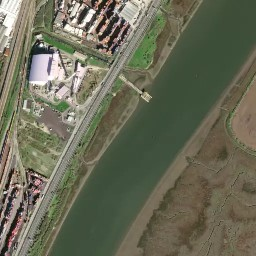
\includegraphics[width=\textwidth]{content/img/datensatz_satellite.jpg}
        \caption{Satellitenbild}
    \end{subfigure}
    \begin{subfigure}{0.2\textwidth}
        \centering
        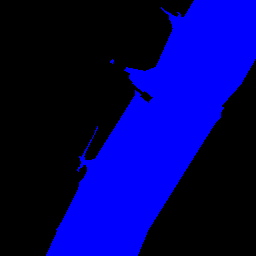
\includegraphics[width=\textwidth]{content/img/datensatz_mask.png}
        \caption{Maske}
    \end{subfigure}
    \caption{Beispiel aus dem Datensatz für ein Satellitenbild aus Littauen mit zugehöriger Maske. \copyright Mapbox, \copyright OpenStreetMap}
    \label{fig:datensatz}
\end{figure}
\\
Der Datensatz wurde mit Python über die API von Mapbox\cite{mapbox} generiert.
Europa hat einen Wasserflächenanteil von wenigen Prozent.
Um nun nicht größtenteils gewässerfreie Satellitenaufnahmen zu erhalten, muss geprüft werden ob sich in den gezogenen Koordinaten ein Fluss, See oder Meer befindet.
Die Erzeugung des Datensatzes kann in folgende Schritte unterteilt werden:
\begin{itemize}
    \item generiere gleichverteilte Längen- und Breitengrade auf dem europäischen Festland (Ländergrenzen aus Natural Earth Datensatz \cite{naturalearth})
    \item prüfe ob Gewässer innerhalb eines 'Tiles'\footnote{\label{foot:tiles}Die Karte wird Abhängig von der Zoomstufe $Z$ in $4^Z$ Quadrate unterteilt, sog. 'Tiles'.} vorkommen über die Mapbox API\cite{mapbox}
    \item Download des Satelliten- und Maskenbildes über die Mapbox API\cite{mapbox} \\
          per Link: \url{https://api.mapbox.com/v4/mapbox.satellite/{zoom}/{lon}/{lat}.mvt?access_token={token}}
    \item skaliere Bilder von $(256 \times 256)$px zu $(128 \times 128)$px
\end{itemize}
Die zufällig erzeugten Längen- und Breitengrade werden im Bereich
\begin{align*}
    \SI{-10.49}{\degree} &< \text{Längengrad} < \SI{40.27}{\degree} \\
    \SI{34.51}{\degree} &< \text{Breitengrad} < \SI{71.20}{\degree}
\end{align*}
gezogen, somit wird Russland und Island im Vorhinein ausgeschlossen.
In dem vorliegenden Bild, welches einem Tile entspricht muss Wasser vorhanden sein.
Zusätzlich darf das Satellitenbild nicht ausschließlich Wasser enthalten, um so redundante Bilder zu vermeiden.
Die Längen- und Breitengrade werden akzeptiert, wenn dies zutrifft und die Koordinaten nicht bereits verwendet wurden.
Das auf der Aufnahme abgebildete Land wird mittels der Koordinaten ermittelt.
\\
Zum Herunterladen der Bilder müssen die zuvor generierten Längen- und Breitengrade und zum anderen der Zoom-Faktor angegeben werden.
Umso größer der Zoom-Faktor, desto kleinere Gewässer können erkannt werden, doch desto größer ist die Wahrscheinlichkeit Satellitenbilder auschließlich mit Wasser zu erhalten.
Mit dem gewählten Zoom-Faktor $Z = 15$ liegt der Fokus auf Flüsse, mittelgroße/große Seen und Küstenabschnitte.
\\
Um die Laufzeit zu verkürzen wird die Anzahl der Pixel pro Bild um $\SI{75}{\percent}$ reduziert.
Die Farbwerte des Satellitenbilds werden auf Werte zwischen $0$ und $1$ normiert.
Während die Pixel des Maskenbilds mit Werten im Bereich $[0, 1]$, per Schwellenwert ($0.5$) in binäre Werte umgerechnet werden.

\subsection{Eigenschaften}
Der Datensatz beinhaltet $\SI{57931}{}$ Einträge mit jeweils folgenden Informationen:
\\
Längengrad, Breitengrad, Name des Landes, Satellitenbild, Maskenbild
\\

\begin{wrapfigure}{r}{7.5cm}
    \centering
    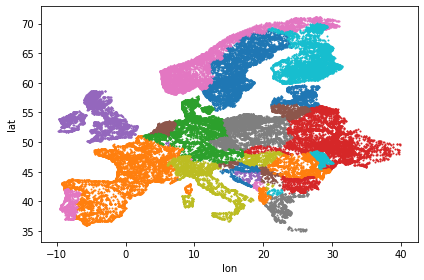
\includegraphics[scale=0.5]{content/img/map.png}
    \caption{Orte der Satellitenbilder, dargestellt als Karte.}
\end{wrapfigure}
\FloatBarrier
Dabei erhält das Modell das Satellitenbild als Eingabe in der Form $(128, 128, 3)$ und die Maske als Ziel in der Form $(128, 128, 1)$.
Die anderen Attribute geben den Ort der Aufnahme an, sind aber nicht für die eigentliche Problemstellung, sondern für die Reproduzierbarkeit notwendig.
\\
Das Satellitenbild liegt im JPEG-Format vor, beinhaltet also die drei Farbkanäle $RGB$ mit Werten von $0$ bis $255$, bzw. nach der Normierung von $0$ bis $1$.
\\
Hingegen wird für das Maskenbild das 'PNG'-Format verwendet.
Es handelt sich um Graustufenbilder mit einem Farbkanal, welcher hier den Wert $1$ für Wasser bzw. $0$ für kein Wasser annehmen kann.
\\
Wie bereits erwähnt, beträgt die Auflösung für Masken- und Satellitenbild $128 \, \text{px} \times 128 \, \text{px}$.